

\documentclass[10pt,twocolumn,letterpaper]{article}

%%%%%%%%% PAPER TYPE  - PLEASE UPDATE FOR FINAL VERSION
% \usepackage{cvpr}              % To produce the CAMERA-READY version
% \usepackage[review]{cvpr}      % To produce the REVIEW version
\usepackage[pagenumbers]{cvpr} % To force page numbers, e.g. for an arXiv version
\usepackage{graphicx}     
\usepackage{subcaption}   
\usepackage{multirow}
\usepackage{tabularx}
\usepackage{booktabs}
\usepackage{colortbl}
\usepackage{amsmath}

% Import additional packages in the preamble file, before hyperref
% \usepackage{amsmath}
% \usepackage{amssymb}
\usepackage{graphicx}
\usepackage{mathtools}
% \mathtoolsset{showonlyrefs}
\usepackage{amsfonts}
% \usepackage{amsthm,bm}
\usepackage{color}
% \usepackage{enumitem}
\usepackage{dsfont}
% \usepackage{pgfplots}
% \pgfplotsset{width=10cm,compat=1.9}
%  \usepackage{pifont}%http://ctan.org/pkg/pifont
\usepackage{thmtools} 
% \usepackage{thm-restate}
% \usepackage{sidecap}

\declaretheorem[name=Theorem]{thm}
\declaretheorem[name=Proposition]{prop}
\declaretheorem[name=Corollary]{cor}


\newcommand{\cmark}{\ding{51}}%
\newcommand{\xmark}{\ding{55}}%
\newcommand{\R}{\mathbb{R}}
\newcommand{\upmark}{\ding{218}}
\newcommand{\downmark}{\ding{216}}
\newcommand{\norm}[1]{\lVert#1\rVert}
\newcommand{\dotprod}[1]{\langle #1\rangle}
\newcommand{\E}{\mathbb{E}} 
\newcommand{\Et}[1]{\mathbf{E}_t\left[#1\right] } 
\newcommand{\Ev}[1]{\mathbf{E}_v\left[#1\right] } 
\newcommand{\EE}[2]{\mathbf{E}_{#1}\left[#2\right] } 
\newcommand{\Prb}[1]{\mathbf{P}\left[#1\right] }
\newcommand{\Tr}[1]{\mathrm{Tr}( #1)}
\newcommand{\Rea}[1]{\mathrm{Re}[ #1]}
\newcommand{\Ima}[1]{\mathrm{Im}[ #1]}
\newcommand{\eqdef}{\overset{\text{def}}{=}} 
\newcommand{\floor}[1]{\lfloor #1 \rfloor}
\newcommand{\Cov}[1]{\mathrm{Cov}\left[#1\right]}
\newcommand{\Var}[1]{\mathrm{Var}\left[#1\right]}
%\newcommand{\argmin}[1]{\underset{#1}{\text{argmin }}  } 
\newcommand{\breg}[2]{\mathcal{D}_{\Phi}\left(#1,#2\right) }
\newcommand{\xx}{\mathbf{x}}
\newcommand{\yy}{\mathbf{y}}
\newcommand{\zz}{\mathbf{z}}
\newcommand{\hmu}{\hat{\mu}}
\renewcommand{\phi}{\varphi}

%\usepackage{algorithm}
%\usepackage[noend]{algpseudocode}

\newcommand{\carles}[1]{{\color{red}{\bf[Carles:} #1{\bf]}}}
\newcommand{\ricky}[1]{{\color{magenta}{\bf[Ricky:} #1{\bf]}}}
\newcommand{\brian}[1]{{\color{orange}{\bf[Brian:} #1{\bf]}}}

% \newcommand{\carles}[1]{}
% \newcommand{\ricky}[1]{}
% \newcommand{\brian}[1]{}

\setlength{\parskip}{0.5em}
\setlength\parindent{0pt}

\graphicspath {{figures/}}

\newcommand{\N}{\mathbb{N}}
\newcommand{\Ff}{\mathcal{F}}
\newcommand{\Gg}{\mathcal{G}}
\usepackage{hyperref}
\usepackage{caption}
\usepackage[super]{nth}
\delimitershortfall-1sp

\newtheorem{lemma}{Lemma}
\newtheorem{definition}{Definition}
\newtheorem{theorem}{Theorem}
\newtheorem{note}{Note}
\newtheorem{assumption}{Assumption}
\newtheorem{proposition}{Proposition}
\newtheorem{example}{Example}
\newtheorem{remark}{Remark}
\newtheorem{corollary}{Corollary}
\newtheorem{observation}{Observation}
% \newtheorem{algorithm}{Algorithm}
\usepackage{subcaption}
%\newcommand{\corollaryautorefname}{Corollary}

\DeclareMathOperator*{\argmin}{argmin}
\DeclareMathOperator*{\argmax}{argmax}

\DeclarePairedDelimiter\abs{\lvert}{\rvert}

\renewcommand{\sectionautorefname}{Sec.}
\renewcommand{\subsectionautorefname}{Subsec.}
\renewcommand{\appendixautorefname}{App.}
\renewcommand{\theoremautorefname}{Thm.}
\renewcommand{\propositionautorefname}{Prop.}
\renewcommand{\corollaryautorefname}{Cor.}
% \renewcommand(\algorithmautorefname}{Alg.}

\newenvironment{talign*}
 {\let\displaystyle\textstyle\csname align*\endcsname}
 {\endalign}
\newenvironment{talign}
 {\let\displaystyle\textstyle\csname align\endcsname}
 {\endalign}

\makeatletter
\renewcommand{\thealgorithm}{\arabic{algorithm}}
% \@addtoreset{algorithm}{chapter}  % Remove or modify this line if you do not want to reset with chapters
\makeatother

\makeatletter
\DeclareRobustCommand{\cev}[1]{%
  {\mathpalette\do@cev{#1}}%
}
\newcommand{\do@cev}[2]{%
  \vbox{\offinterlineskip
    \sbox\z@{$\m@th#1 x$}%
    \ialign{##\cr
      \hidewidth\reflectbox{$\m@th#1\vec{}\mkern4mu$}\hidewidth\cr
      \noalign{\kern-\ht\z@}
      $\m@th#1#2$\cr
    }%
  }%
}
\makeatother

\definecolor{mygray}{gray}{0.95}
\newcommand{\greybox}[1]{
\vspace{-0.9em}
\begin{center}			% Centering minipage
\vspace{-0.5em}
\colorbox{mygray} {		% Set's the color of minipage
\begin{minipage}{0.987\linewidth} 	% Starts minipage
\centering
\vspace{-0.8em}
{#1}
\end{minipage}}			% End minipage
\end{center}
\vspace{-0.5em}
}

% It is strongly recommended to use hyperref, especially for the review version.
% hyperref with option pagebackref eases the reviewers' job.
% Please disable hyperref *only* if you encounter grave issues, 
% e.g. with the file validation for the camera-ready version.
%
% If you comment hyperref and then uncomment it, you should delete *.aux before re-running LaTeX.
% (Or just hit 'q' on the first LaTeX run, let it finish, and you should be clear).
\definecolor{cvprblue}{rgb}{0.21,0.49,0.74}
\usepackage[pagebackref,breaklinks,colorlinks,allcolors=cvprblue]{hyperref}


%%%%%%%%% TITLE - PLEASE UPDATE
\title{Timestep Embedding Tells: It's Time to Cache for Video Diffusion Model}

%%%%%%%%% AUTHORS - PLEASE UPDATE
\author{Feng Liu\textsuperscript{1}\thanks{Work was done during internship at Alibaba Group
.}\quad 
Shiwei Zhang\textsuperscript{2}\quad
Xiaofeng Wang\textsuperscript{1,3}\quad
Yujie Wei\textsuperscript{4}\quad
Haonan Qiu\textsuperscript{5}\\
Yuzhong Zhao\textsuperscript{1}\quad
Yingya Zhang\textsuperscript{2}\quad
Qixiang Ye\textsuperscript{1}\quad
Fang Wan\textsuperscript{1}\thanks{Corresponding author.}\\
\textsuperscript{1}University of Chinese Academy of Sciences
\quad
\textsuperscript{2}Alibaba Group\\
\textsuperscript{3}Institute of Automation, Chinese Academy of Sciences\\
\textsuperscript{4}Fudan University\quad
\textsuperscript{5}Nanyang Technological University\\
Project Page: {\color{magenta}https://liewfeng.github.io/TeaCache}}

\begin{document}
\maketitle
\begin{abstract}
We introduce Causal Diffusion as the autoregressive (AR) counterpart of Diffusion models. It is a next-token(s) forecasting framework that is friendly to both discrete and continuous modalities and compatible with existing next-token prediction models like LLaMA and GPT. While recent works attempt to combine diffusion with AR models, we show that introducing sequential factorization to a diffusion model can substantially improve its performance and enables a smooth transition between AR and diffusion generation modes. Hence, we propose \textbf{CausalFusion} - a decoder-only transformer that dual-factorizes data across sequential tokens and diffusion noise levels, leading to state-of-the-art results on the ImageNet generation benchmark while also enjoying the AR advantage of generating an arbitrary number of tokens for in-context reasoning. We further demonstrate CausalFusion's multimodal capabilities through a joint image generation and captioning model, and showcase CausalFusion's ability for zero-shot in-context image manipulations. We hope that this work could provide the community with a fresh perspective on training multimodal models over discrete and continuous data.
\end{abstract}    
\vspace{-10pt}
\section{Introduction}
\label{sec:intro}
Autoregressive (AR) and diffusion models are two powerful paradigms for data distribution modeling. AR models, also known as the next token prediction approach, dominate language modeling and are considered central to the success of large language models (LLMs)~\cite{gpt1,gpt2,gpt3,llama1,llama2,llama3}. On the other hand, diffusion models~\cite{ddpm,dit,adm,edm}, or score-based generative models~\cite{songscore,lipman2023flow}, have emerged as the leading approach for visual generation, driving unprecedented progress in the era of visual content generation~\cite{sora,rombach2022high,li2023scaling}. 

\begin{figure}[t]
    \centering
    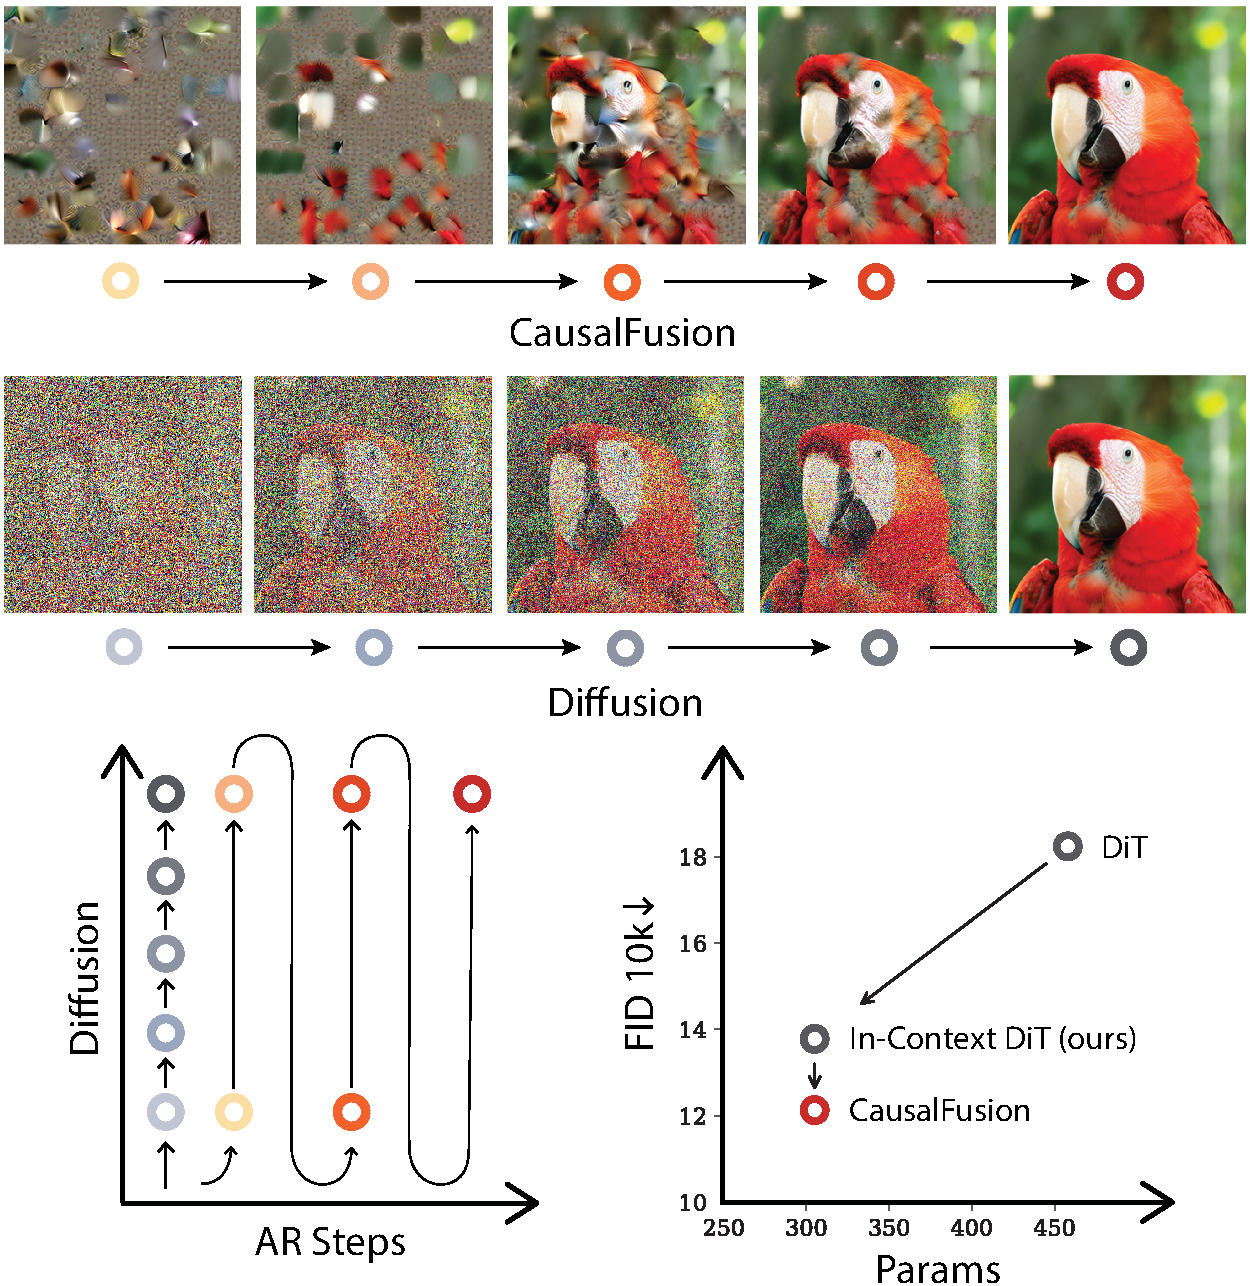
\includegraphics[width=1.0\textwidth,height=1.0\textwidth]{figs/casualfusion-teaser-v6.pdf} 
    \vspace*{-6mm}
    \caption{
    \textbf{Illustration of Dual-Factorization}. The arrow line indicates CausalFusion's generation path, moving from one state to the next by jointly generating along the sequential and noise-level dimension at each step. 
    Compared to DiT, our In-context DiT substantially improves results with fewer parameters. CausalFusion further enhances performance without changing the architecture or parameter count. Results were trained on IN1K for 240 epochs. CausalFusion adopts arbitrary AR steps for image generation, but each step only diffuses partial tokens, resulting in similar (or slightly lower) computational complexity.
    \vspace{-10pt}
    }
    \label{fig:dual-factorization}
\end{figure}


\begin{figure*}[t]
  \centering
  \begin{subfigure}{1.0\linewidth}
    \centering
    \includegraphics[width=\linewidth]{figs/figure2.pdf}
    \caption{Samples generated by CausalFusion-XL/2, ImageNet 512$\times$512, 800 epoch, DDPM 250 steps, CFG=4.0}
  \end{subfigure}
  \begin{subfigure}{1.0\linewidth}
    \centering
    \includegraphics[width=\linewidth]{figs/edit.pdf}
    \caption{\textbf{Zero-shot image editing} results generated by CausalFusion-XL/2, ImageNet 512$\times$512, 800 epoch. We first generate the original image (those on the left), then mask out its centre region, top-half, or bottom-half, and regenerate the image with new class conditions. Details are discussed in Sec \ref{sec:system}.}
  \end{subfigure}
  \caption{\textbf{Visualization results}. All samples are generated by models trained only on \textbf{ImageNet-1K class-conditional generation} task, demonstrating CausalFusion's zero-shot image manipulation ability. See more visualization results in Appendix~\ref{appendix:secD}.
  \vspace{-12pt}
  }
  \vspace{-6pt}
  \label{fig:vis1}
\end{figure*}

The intrinsic distinction between AR and diffusion models lies in their approach to data distribution factorization. AR models treat data as an ordered sequence, factorizing it along the sequential axis, where the probability of each token is conditioned on all preceding tokens. This factorization enables the AR paradigm to generalize effectively and efficiently across arbitrary number of tokens, making it well-suited for long-sequence reasoning and in-context generation. In contrast, diffusion models factorize data along the noise-level axis, where the tokens at each step are a refined (denoised) version of themselves from the previous step. As a result, the diffusion paradigm is generalizable to arbitrary number of data refinement steps, enabling iterative quality improvement with scaled inference compute. While AR and diffusion models each excel within their respective domains, their distinct factorization approaches reveal complementary potential. Although recent studies~\cite{transfusion,monoformer,dart} have attempted to integrate AR and diffusion within a single model, they typically treat these paradigms as separate modes, missing the potential benefits of jointly exploring them within a 2-D factorization plane.

To this end, we introduce \textbf{CausalFusion}, a flexible framework that integrates both sequential and noise-level data factorization to unify their advantages. The degree of factorization along these two axes—namely, the AR step and diffusion step—is adjustable, enabling {CausalFusion} to revert seamlessly to the traditional AR or diffusion paradigms at either extreme. To enhance its generality, CausalFusion is designed to predict \textit{any} number of tokens at \textit{any} AR step, with \textit{any} pre-defined sequence order and \textit{any} level of inference compute, thereby minimizing the inductive biases presented in existing generative models. As shown in Figure~\ref{fig:dual-factorization}, this approach provides a broad spectrum between the AR and diffusion paradigms, allowing smooth interpolation within two endpoints during both training and inference. 
Specifically, we explore CausalFusion in image generation and multimodal generation scenarios, where we observe that the level of training difficulties significantly influences the overall effectiveness of CausalFusion.

\textbf{Difficulties of generative tasks in CausalFusion:} Both AR and diffusion paradigms present unique challenges based on difficulties of their specific generative stages. In diffusion models, the effectiveness of training depends heavily on proper loss weighting across noise levels~\cite{ddpm,minsnr}, as higher noise levels are more difficult and usually provide more valuable signals than lower noise levels. Similarly, AR models are susceptible to error accumulation~\cite{bengio2015scheduled} as early-stage predictions are made with limited visible context, making them more error-prone. Optimizing CausalFusion thus requires balancing across these varying task difficulties to optimize training signal impact and ensure sufficient exploration across the entire factorization plane.

In this paper, we formally examine the difficulties of generative tasks within CausalFusion. We show that, in addition to the noise levels in diffusion and the amount of visible context in AR, the total number of AR steps, which controls the interpolation between AR and diffusion, also plays a critical role in shaping training difficulties. Driven by these factors, we develop a scalable and versatile model based on the CausalFusion framework. Starting from the DiT architecture~\cite{dit}, we gradually convert it into a decoder-only transformer compatible with existing AR models like GPT~\cite{gpt1,gpt2,gpt3} and LLaMA~\cite{llama1,llama2,llama3}. We provide insights on how to appropriately choose the number of AR steps during the training of CausalFusion models, and further introduce loss weighing along both the diffusion and AR axis to balance the impact of different generative stages. As shown in Figure~\ref{fig:dual-factorization} and ~\ref{fig:vis1}, our model achieves state-of-the-art performance on the ImageNet class-conditional generation benchmark, significantly outperforming DiT~\cite{dit} and enabling zero-shot image manipulations due to its AR nature. When pretraining on both text-to-image and image-to-text tasks, our model surpasses forced-fusion frameworks such as TransFusion~\cite{transfusion}, demonstrating the versatility of our CausalFusion framework.


We highlight our main contribution below:
\begin{itemize}
\item  We propose CausalFusion as the AR counterpart to DiT, achieving state-of-the-art results and enabling the unlimited token generation for in-context reasoning.
\item  We systematically study CausalFusion on the dual-factorization plane and identify key factors that improve the effectiveness of CausalFusion models.
\item  Compared with recent studies~\cite{transfusion}, CausalFusion enables a smooth, cohesive integration with language modeling for cross-modal generation and reasoning.
\end{itemize} 

\section{Related Work}
\label{sec:related}                             

\noindent{\textbf{Text-to-Video Generation.}}~Early video generation models were primarily based on Unet-based latent diffusion models (LDMs) extended from text-to-image models like Stable Diffusion~\cite{rombach2022high}. For example, AnimateDiff~\cite{guo2023animatediff} introduced a temporal attention module to improve temporal consistency across frames. Subsequent video generation models~\cite{wang2023modelscope, cerspense2023zeroscope, chen2023videocrafter1, chen2024videocrafter2, zhang2024moonshot, zhang2023show} adopted an alternating approach with 2D spatial and 1D temporal attention, including works like ModelScope, VideoCrafter, Moonshot, and Show-1. 

With advancements in large language models (LLMs) and the introduction of Sora~\cite{sora2024}, attention shifted from Unet architectures to transformer-based architectures (DiT). DiT-based video generation models, such as Latte~\cite{ma2024latte} and OpenSora~\cite{opensora}, extended the DiT text-to-image (T2I) model~\cite{chen2023pixart} and maintained the 2D and 1D alternating attention approach, achieving promising results. Recently, DiT-based video generation has rapidly progressed, achieving further improvements in quality. Several methods~\cite{yang2024cogvideox, opensoraplan, genmo2024mochi} have moved away from the 2D and 1D alternating approach, instead treating video frames as a single long sequence with 3D positional embeddings for encoding. These approaches also prepend text tokens—processed through a text encoder—to the video sequence, creating a streamlined network that relies solely on full self-attention and feed-forward layers. Our method builds upon these recent open-source transformer-based video generation models.


\vspace{0.5em}
\noindent{\textbf{Video Matting.}}~A straightforward approach for RGBA video generation is to extract the alpha channel from generated RGB content, as done with traditional green screen keying or learning-based video matting expert models~\cite{lin2023omnimatterf, lin2021real, lin2022robust}. OmnimatteRF~\cite{lin2023omnimatterf} introduces a video matting method that combines dynamic 2D foreground layers with a 3D background model, enabling more realistic scene reconstruction for real-world videos. Robust Video Matting (RVM)~\cite{lin2022robust} proposes a real-time, high-quality human video matting method with a recurrent architecture for improved temporal coherence, achieving state-of-the-art results without auxiliary inputs. Another work presents a high-speed, high-resolution background replacement technique with precise alpha matte extraction, supported by the VideoMatte240K and PhotoMatte13K/85 datasets~\cite{lin2021real}. Additionally, many image matting methods~\cite{chen2022pp, li2024matting, yao2024vitmatte, wang2024matting} can be applied for frame-by-frame matting.


Further, several works~\cite{he2024lotus, yang2024depth, ke2024repurposing} in image depth estimation adapt pretrained generation models for prediction tasks, achieving strong performance that often surpasses traditional, scratch-trained expert models. Marigold~\cite{ke2024repurposing} modifies architectures to create image-conditioned generation models, while Lotus~\cite{he2024lotus} explores the role of the diffusion process in this context. Although there is currently no dedicated approach for video matting within video generation models, we replicate and extend these methods to evaluate their performance, allowing us to highlight the limitations of prediction-based pipelines for RGBA generation.

\vspace{0.5em}
\noindent{\textbf{Generation beyond RGB.}}~Another category of methods~\cite{zhang2024transparent, long2024wonder3d, bao2023one, luo2024intrinsicdiffusion, zeng2024rgb, he2024lucidfusion, yang2023defect} explores expanding generation models to simultaneously generate additional channels, though they are not specifically designed for RGBA video generation. 
For instance, LayerDiffusion~\cite{zhang2024transparent} modifies the VAE in latent diffusion models to decode alpha channels. However, VAEs typically lack the semantic understanding required for precise alpha generation, limiting their effectiveness in complex visual scenarios where texture and contour details are critical. 
In contrast, other approaches~\cite{long2024wonder3d, bao2023one, luo2024intrinsicdiffusion, zeng2024rgb} modify the denoising model directly to enable joint generation. Wonder3D~\cite{long2024wonder3d} uses a domain embedding to control the model’s generation modality, while methods like IntrinsicDiffusion~\cite{luo2024intrinsicdiffusion} and RGB\(\leftrightarrow\)X~\cite{zeng2024rgb} adapt the UNet’s input and output layers to jointly produce intrinsic modalities. However, all these methods are designed for image tasks and rely on UNet architectures. When applied to video generation, they face limitations in quality and diversity due to the scarcity of RGBA video data.

\section{Method}
%%%%%%%%% Figure: Overall framework
\begin{figure*}[t]
  \centering
   \includegraphics[width=0.85\linewidth]{figures/PoolFormer_overall_architecture.pdf}
   \vspace{-4mm}
   \caption{\textbf{(a) The overall framework of \modelname{}.} Similar to \cite{resnet, pvt, swin}, \modelname{} adopts hierarchical architecture with 4 stages. For a model with L \modelname{} blocks, stage [1, 2, 3, 4] have [L/6, L/6, L/2, L/6] blocks, respectively. The feature dimension $D_i$ of stage $i$ is shown in the figure. \textbf{(b) The architecture of \modelname{} block.} Compared with Transformer block, it replaces attention with extremely simple non-parametric operator, pooling, to conduct only basic token mixing.}
   \label{fig:overall_architecture}
\end{figure*}


%%%%%%%%% Algorithm: Pooling
\begin{algorithm}[t]
\caption{Pooling for PoolFormer, PyTorch-like Code}
\label{alg:code}
\definecolor{codeblue}{rgb}{0.25,0.5,0.5}
\definecolor{codekw}{rgb}{0.85, 0.18, 0.50}
\lstset{
  backgroundcolor=\color{white},
  basicstyle=\fontsize{7.5pt}{7.5pt}\ttfamily\selectfont,
  columns=fullflexible,
  breaklines=true,
  captionpos=b,
  commentstyle=\fontsize{7.5pt}{7.5pt}\color{codeblue},
  keywordstyle=\fontsize{7.5pt}{7.5pt}\color{codekw},
}
\begin{lstlisting}[language=python]
import torch.nn as nn

class Pooling(nn.Module):
    def __init__(self, pool_size=3):
        super().__init__()
        self.pool = nn.AvgPool2d(
            pool_size, stride=1, 
            padding=pool_size//2, 
            count_include_pad=False,
        )
    def forward(self, x):
        """
        [B, C, H, W] = x.shape
        Subtraction of the input itself is added 
        since the block already has a 
        residual connection.
        """
        return self.pool(x) - x
\end{lstlisting}
\end{algorithm}

\subsection{MetaFormer}
We present the core concept ``MetaFormer" for this work at first. As shown in Figure \ref{fig:first_figure}, abstracted from Transformers \cite{transformer}, 
MetaFormer is a general architecture where the token mixer is not specified while the other components are kept the same as Transformers. The input $I$ is first processed by input embedding, such as  patch embedding for ViTs \cite{vit},
\begin{equation}
    X = \mathrm{InputEmb}(I),
\end{equation}
where  $X \in \mathbb{R}^{N \times C}$ denotes the embedding tokens with sequence length $N$ and embedding dimension $C$. 


Then, embedding tokens are fed to repeated MetaFormer blocks, each of which includes two residual sub-blocks. Specifically, the first sub-block mainly contains a token mixer to communicate information among tokens and this sub-block can be expressed as
\begin{equation}
    Y = \mathrm{TokenMixer}(\mathrm{Norm}(X)) + X,
\end{equation}
where $\mathrm{Norm}(\cdot)$ denotes the normalization such as Layer Normalization \cite{layer_norm} or Batch Normalization \cite{batch_norm}; $\mathrm{TokenMixer}(\cdot)$ means a module mainly working for mixing token information. It is implemented by various attention mechanism in recent vision Transformer models  \cite{vit,refiner,t2t} or spatial MLP in MLP-like models \cite{mlp-mixer, resmlp}. Note that the main function of the token mixer is to propagate token information although some token mixers can also mix channels, like attention. 


The second sub-block primarily consists of a two-layered MLP with non-linear activation, 
\begin{equation}
    Z = \sigma(\mathrm{Norm}(Y)W_1)W_2 + Y,
\end{equation}
where $W_1 \in \mathbb{R}^{C \times rC}$ and $W_2 \in \mathbb{R}^{rC \times C}$ are learnable parameters with MLP expansion ratio $r$; $\sigma(\cdot)$ is a non-linear activation function, such as GELU \cite{gelu} or ReLU \cite{relu}. 

\myPara{Instantiations of MetaFormer} MetaFormer describes a general architecture 
% a general architecture that is powerful at solving computer vision tasks.  
with which different models can be obtained immediately by specifying the concrete design of the token mixers. 
As shown in Figure \ref{fig:first_figure}(a), if the token mixer is specified as attention or spatial MLP, MetaFormer then becomes a Transformer or MLP-like model respectively. 

\subsection{PoolFormer}
From the introduction of Transformers \cite{transformer}, lots of works attach much importance to the attention and focus on designing various attention-based token mixer components. In contrast, these works pay little attention to the general architecture, \ie, the MetaFormer.


In this work, we argue that this MetaFormer general architecture contributes mostly to the success of the recent Transformer and MLP-like models. 
To demonstrate it, we deliberately employ an embarrassingly simple operator, pooling, as the token mixer. This operator has no learnable parameters and it just makes each token averagely aggregate its nearby token features. 


Since this work is targeted at vision tasks,  we assume the input is in channel-first data format, \ie,  $T \in \mathbb{R}^{C \times H \times W}$. The pooling operator can be expressed as
\begin{equation}
\label{eq:pool}
    T'_{:, i, j} =  \frac{1}{K \times K} \sum_{p,q=1}^{K}T_{:, i+p-\frac{K+1}{2}, i+q-\frac{K+1}{2}} - T_{:, i, j},
\end{equation}
where $K$ is the pooling size. Since the MetaFormer block already has a residual connection, subtraction of the input itself is added in Equation (\ref{eq:pool}). The PyTorch-like code of the pooling is shown in Algorithm \ref{alg:code}.


As well known, self-attention and spatial MLP have computational complexity quadratic to the number of tokens to mix. Even worse, spatial MLPs bring much more parameters when handling longer sequences. As a result, self-attention and spatial MLPs usually can only process hundreds of tokens. In contrast, the pooling needs a computational complexity linear to the sequence length without any learnable parameters.  Thus, we take advantage of pooling by adopting a hierarchical structure similar to traditional CNNs \cite{alexnet, vgg, resnet} and recent hierarchical Transformer variants \cite{swin, pvt}. Figure \ref{fig:overall_architecture} shows the overall framework of PoolFormer. Specifically, PoolFormer has 4 stages with $\frac{H}{4} \times \frac{W}{4}$, $\frac{H}{8} \times \frac{W}{8}$, $\frac{H}{16} \times \frac{W}{16}$, and $\frac{H}{32} \times \frac{W}{32}$ tokens respectively, where $H$ and $W$ represent the width and height of the input image. There are two groups of embedding size: 1) small-sized models with embedding dimensions of 64, 128, 320, and 512 responding to the four stages; 2) medium-sized models with embedding dimensions 96, 192, 384, and 768. Assuming there are $L$ PoolFormer blocks in total, stages 1, 2, 3, and 4 will contain $L/6$, $L/6$, $L/2$, and $L/6$ PoolFormer blocks respectively. The MLP expansion ratio is set as 4. According to the above simple model scaling rule, we obtain 5 different model sizes of PoolFormer and their hyper-parameters are shown in Table \ref{tab:model}.


%%%%%%%%% Table: Model Configurations
\begin{table}[t]
\footnotesize
\centering
\setlength{\tabcolsep}{2pt}
% \scalebox{0.65}{\newcommand{\blockc}[4]{
$\begin{bmatrix}
	\begin{array}{l}
	R_1=#1 \\
	N_1=#2 \\
	E_1=#3 \\
	\end{array}
\end{bmatrix} \times #4$
}

\newcommand{\sblock}[3]{
$\begin{matrix}
E_{#1}=#2 \\
L_{#1}=#3 \\
\end{matrix}$
}

\newcommand{\poollayer}{
Pooling Size & \multicolumn{5}{c}{$3 \times 3$, stride 1}\\
\cline{4-9}
}

\newcommand{\stitle}[6]{
\multirow{5}{*}{#1} & \multirow{5}{*}{\scalebox{1}{$\frac{H}{#2}\times \frac{W}{#2}$}} & \multirow{2}{*}{\tabincell{c}{Patch \\ Embedding}} & Patch Size & \multicolumn{5}{c}{$#3 \times #3$, stride $#4$} \\
\cline{4-9}
    &    &    & Embed. Dim. & \multicolumn{3}{c|}{$#5$} & \multicolumn{2}{c}{$#6$} \\
\cline{3-9}
& & \multirow{3}{*}{\tabincell{c}{\modelname{}\\Block}} 
}

\begingroup
\renewcommand{\arraystretch}{1.1}
\begin{tabular}{c|c|c|c|c|c|c|c|c}
\toprule
  \multirow{2}{*}{Stage} & \multirow{2}{*}{\#Tokens} & \multicolumn{2}{c|}{\multirow{2}{*}{Layer Specification}} & \multicolumn{5}{c}{\modelname{}} \\
\cline{5-9}
 & & \multicolumn{2}{c|}{} & S12 & S24 & S36 & M36 & M48 \\
\whline
\stitle{1}{4}{7}{4}{64}{96}    & \poollayer
 & & & MLP Ratio & \multicolumn{5}{c}{4} \\
\cline{4-9}
 & & & \# Block & 2 & 4 & 6 & 6 & 8 \\
\hline
\stitle{2}{8}{3}{2}{128}{192}  & \poollayer
 & & & MLP Ratio & \multicolumn{5}{c}{4} \\
 \cline{4-9}
 & & & \# Block & 2 & 4 & 6 & 6 & 8 \\
\hline
\stitle{3}{16}{3}{2}{320}{384} & \poollayer
 & & & MLP Ratio & \multicolumn{5}{c}{4} \\
\cline{4-9}
 & & & \# Block & 6 & 12 & 18 & 18 & 24 \\
\hline
\stitle{4}{32}{3}{2}{512}{768} & \poollayer
 & & & MLP Ratio & \multicolumn{5}{c}{4} \\
 \cline{4-9}
 & & & \# Block & 2 & 4 & 6 & 6 & 8 \\
\hline
\multicolumn{4}{c|}{Parameters~(M)}& 11.9 & 21.4              &  30.8            &  56.1              &  73.4    \\
\hline
\multicolumn{4}{c|}{MACs~(G)}     & 1.8  &  3.4              &  5.0             &  8.8              &  11.6    \\
\bottomrule
\end{tabular}
\endgroup
}
\newcommand{\blockc}[4]{
$\begin{bmatrix}
	\begin{array}{l}
	R_1=#1 \\
	N_1=#2 \\
	E_1=#3 \\
	\end{array}
\end{bmatrix} \times #4$
}

\newcommand{\sblock}[3]{
$\begin{matrix}
E_{#1}=#2 \\
L_{#1}=#3 \\
\end{matrix}$
}

\newcommand{\poollayer}{
Pooling Size & \multicolumn{5}{c}{$3 \times 3$, stride 1}\\
\cline{4-9}
}

\newcommand{\stitle}[6]{
\multirow{5}{*}{#1} & \multirow{5}{*}{\scalebox{1}{$\frac{H}{#2}\times \frac{W}{#2}$}} & \multirow{2}{*}{\tabincell{c}{Patch \\ Embedding}} & Patch Size & \multicolumn{5}{c}{$#3 \times #3$, stride $#4$} \\
\cline{4-9}
    &    &    & Embed. Dim. & \multicolumn{3}{c|}{$#5$} & \multicolumn{2}{c}{$#6$} \\
\cline{3-9}
& & \multirow{3}{*}{\tabincell{c}{\modelname{}\\Block}} 
}

\begingroup
\renewcommand{\arraystretch}{1.1}
\begin{tabular}{c|c|c|c|c|c|c|c|c}
\toprule
  \multirow{2}{*}{Stage} & \multirow{2}{*}{\#Tokens} & \multicolumn{2}{c|}{\multirow{2}{*}{Layer Specification}} & \multicolumn{5}{c}{\modelname{}} \\
\cline{5-9}
 & & \multicolumn{2}{c|}{} & S12 & S24 & S36 & M36 & M48 \\
\whline
\stitle{1}{4}{7}{4}{64}{96}    & \poollayer
 & & & MLP Ratio & \multicolumn{5}{c}{4} \\
\cline{4-9}
 & & & \# Block & 2 & 4 & 6 & 6 & 8 \\
\hline
\stitle{2}{8}{3}{2}{128}{192}  & \poollayer
 & & & MLP Ratio & \multicolumn{5}{c}{4} \\
 \cline{4-9}
 & & & \# Block & 2 & 4 & 6 & 6 & 8 \\
\hline
\stitle{3}{16}{3}{2}{320}{384} & \poollayer
 & & & MLP Ratio & \multicolumn{5}{c}{4} \\
\cline{4-9}
 & & & \# Block & 6 & 12 & 18 & 18 & 24 \\
\hline
\stitle{4}{32}{3}{2}{512}{768} & \poollayer
 & & & MLP Ratio & \multicolumn{5}{c}{4} \\
 \cline{4-9}
 & & & \# Block & 2 & 4 & 6 & 6 & 8 \\
\hline
\multicolumn{4}{c|}{Parameters~(M)}& 11.9 & 21.4              &  30.8            &  56.1              &  73.4    \\
\hline
\multicolumn{4}{c|}{MACs~(G)}     & 1.8  &  3.4              &  5.0             &  8.8              &  11.6    \\
\bottomrule
\end{tabular}
\endgroup

\vspace{-3mm}
\caption{\textbf{ Configurations of different PoolFormer models.} There are two groups of embedding dimensions, \ie, small size with [64, 128, 320, 512] dimensions and medium size with [96, 196, 384, 768]. Notation ``S24" means the model is in small size of embedding dimensions with 24 PoolFormer blocks in total. The numbers of MACs are counted by \texttt{fvcore}\cite{fvcore} library.
}
\label{tab:model}
\vspace{-4mm}
\end{table}




\section{Experiment}

\begin{figure*}
  \centering
  \includegraphics[width=0.98\linewidth]{figs/tisser.pdf}
  \caption{
  Comparison of visual quality and efficiency (denoted by latency) with the competing method. TeaCache outperforms PAB~\cite{zhao2024real} in both visual quality and efficiency. Latency is evaluated on a single A800 GPU. Video generation specifications: Open-Sora~\cite{Open-Sora} (51 frames, 480p), Latte~\cite{ma2024latte} (16 frames, 512$\times$512), Open-Sora-Plan~\cite{Open-Sora-Plan} (65 frames , 512$\times$512). Best-viewed with zoom-in.
  }
  \label{fig:show}
\end{figure*}



\subsection{Settings}
\textbf{Base Models and Compared Methods.} To demonstrate the effectiveness of our method, we apply our acceleration technique to various video, such as Open-Sora 1.2 ~\cite{Open-Sora}, Open-Sora-Plan~\cite{Open-Sora-Plan} and Latte~\cite{ma2024latte}. We compare our base models with recent efficient video synthesis techniques, including PAB~\cite{zhao2024real}, T-GATE~\cite{zhang2024cross} and $\Delta$-DiT~\cite{chen2024delta}, to highlight the advantages of our approach. Notably, $\Delta$-DiT and T-GATE are originally designed as an acceleration method for image synthesis; PAB adapted them for video synthesis to facilitate comparison. 

\textbf{Evaluation Metrics and Datasets.} To assess the performance of video synthesis acceleration methods, we focus on two primary aspects: inference efficiency and visual quality. For evaluating inference efficiency, we use Floating Point Operations (FLOPs) and inference latency as metrics. For visual quality evaluation, we employ VBench~\cite{huang2024vbench}, LPIPS~\cite{zhang2018unreasonable}, PSNR, and SSIM. VBench serves as a comprehensive benchmark suite for video generative models, aligning well with human perceptions and offering valuable insights from multiple perspectives. LPIPS, PSNR, and SSIM evaluate the similarity between videos produced by the accelerated sampling method and the original model. PSNR assesses pixel-level fidelity, LPIPS measures perceptual consistency, and SSIM evaluates structural similarity. Generally, higher similarity scores imply better fidelity and visual quality. The details of evaluation metrics are presented in Appendix.

\textbf{Implementation Detail} All experiments are carried out on the NVIDIA A800 80GB GPUs with Pytorch. We enable FlashAttention~\cite{dao2022flashattention} by default for all experiments.  To obtain robust polynomial fitting, we sample 70 texts from T2V-CompBench~\cite{sun2024t2v} to generate videos, assessing seven desired attributes of generated videos. 10 prompts are sampled for each attributes.
$\delta$ is 0.1 for TeaCache-slow and 0.2 for TeaCache-fast.


\begin{figure*}
    \centering
    \begin{minipage}{\textwidth}
    \centering
    \begin{subfigure}{0.24\textwidth}
        \centering
        \includegraphics[width=\textwidth]{figs/480_48.pdf} 
        \caption{480P, 48 frames}
    \end{subfigure}
    \hfill
    \begin{subfigure}{0.24\textwidth}
        \centering
        \includegraphics[width=\textwidth]{figs/480_192.pdf} 
        \caption{480P, 192 frames}
    \end{subfigure}
    \hfill
    \begin{subfigure}{0.24\textwidth}
        \centering
        \includegraphics[width=\textwidth]{figs/360_240.pdf}
        \caption{360P, 240 frames}
    \end{subfigure}
    \hfill
    \begin{subfigure}{0.24\textwidth}
        \centering
        \includegraphics[width=\textwidth]{figs/720_48.pdf}
        \caption{720P, 48 frames}
    \end{subfigure}

    \end{minipage}

    \caption{Inference efficiency and visual quality of TeaCache at different video lengths and resolutions.}
    \label{fig:multi resolution}
\end{figure*}



\subsection{Main Results}

\textbf{Quantitative Comparison.} Tab.~\ref{tab: main} presents a quantitative evaluation of efficiency and visual quality using the VBench benchmark ~\cite{huang2024vbench}. We examine two variants of TeaCache: a slow variant and a fast variant with greater speedup. Compared to other training-free acceleration methods, TeaCache consistently achieves superior efficiency and better visual quality across different base models, sampling schedulers, video resolutions, and lengths. In evaluating the Latte~\cite{ma2024latte} baseline, the TeaCache-slow model demonstrates superior performance across all visual quality metrics, achieving a 1.86× speedup compared to PAB~\cite{zhao2024real}, which provides a 1.34× speedup. TeaCache-fast achieves the highest acceleration at 3.28×, albeit with a slight reduction in visual quality. With the OpenSora~\cite{Open-Sora} baseline, we obtain the optimal speedup of 2.25× as compared to the previous 1.40×, and the highest overall quality with a speedup of 1.55×. Additionally, using Open-Sora-Plan~\cite{Open-Sora-Plan}, TeaCache achieves the highest speedup of 6.83×, surpassing the previously best 1.49× offered by PAB, while also delivering the highest quality at a speedup of 4.41×.


\textbf{Visualization.} Fig.~\ref{fig:show} compares the videos generated by TeaCache against those by the original model and  PAB. The results demonstrate that TeaCache outperforms PAB in visual quality with lower latency. More visual results can be found in the Appendix.

\subsection{Ablation Studies}




\textbf{Scaling to multiple GPUs.} Aligned with previous research employing Dynamic Sequence Parallelism (DSP)~\cite{zhao2024real} for supporting high-resolution long-video generation across multiple GPUs, we assess the performance of TeaCache in these scenarios.  
The results of this study are presented in Tab.~\ref{tab: multiple GPU}. We utilize Open-Sora~\cite{Open-Sora} (480p - 192 frames at 30 timesteps) and Open-Sora-Plan~\cite{Open-Sora-Plan} (512×512 - 221 frames at 150 timesteps) as baselines and compare them against the prior method PAB~\cite{zhao2024real} regarding latency measurements on A800 GPUs. As the number of GPUs increases, TeaCache consistently improves inference speed across various base models and outperforms PAB. 


\textbf{Performance at different Length and Resolution.} To assess the effectiveness of our method in accelerating sampling for videos with varying sizes, we perform tests across different video lengths and resolutions. The results, presented in Fig.~\ref{fig:multi resolution}, demonstrate that our method sustains consistent acceleration performance, even with increases in video resolution and frame count. This consistency highlights the method's potential to accelerate sampling processes for longer and higher-resolution videos, meeting practical demands.

\textbf{Quality-Efficiency trade-off.} In Fig.~\ref{fig:shot}, we compare the quality-latency trade-off of TeaCache with PAB~\cite{zhao2024real}. Our analysis reveals that TeaCache achieves significantly higher reduction rates, indicated by lower absolute latency, compared to PAB. Additionally, across a wide range of latency configurations, TeaCache consistently outperforms PAB on all quality metrics. This is particularly evident in the reference-free metric VBench score~\cite{huang2024vbench}, which aligns more closely with human preferences. Although there is a decline in reference-based scores such as PSNR and SSIM at extreme reduction rates, qualitative results suggest that the outputs remain satisfactory, despite not perfectly matching the reference.

\textbf{Choice of Indicator.} When determining the caching schedule, we evaluate various indicators to estimate the differences in model outputs across consecutive timesteps. These indicators include timestep embedding and timestep embedding-modulated noisy input. As illustrated in Fig.~\ref{fig:difference}, the timestep embedding-modulated noisy input demonstrates a stronger correlation with model output compared to the timestep embedding, particularly in the OpenSora. Moreover, the selection of timesteps by the timestep embedding-modulated noisy input adapts dynamically to different prompts, whereas the timestep embedding selects the same timesteps for all prompts. This observation is validated by the results presented in Tab.~\ref{tab:indicator}, where the timestep embedding-modulated noisy input consistently surpasses the timestep embedding across various models, especially in OpenSora.

\textbf{Effect of Rescaling.} Tab.\ref{tab:fitting} illustrates the impact of rescaling. A first-order polynomial fitting outperforms the original data by 0.24\% under Vbench score metric, as well as in LPIPS, SSIM, and PSNR metrics. Performance gains tend to saturate with a fourth-order polynomial fitting.




\begin{table}[]
\scriptsize
\centering
    \caption{Ablation study of caching indicator. `Timestep': timestep embedding. `Input': timestep embedding-modulated noisy input.}
    % `Input' consistently outperforms `Timestep' with several models.}
    \label{tab:indicator}
\begin{tabular}{c|cccc}
\toprule
\textbf{Indicator}             &\textbf{VBench $\uparrow$} & \textbf{LPIPS $\downarrow$} & \textbf{SSIM $\uparrow$} & \textbf{PSNR $\uparrow$} \\
\hline
\rowcolor[gray]{0.9}OpenSora              & 79.22\%          &  -         &  -         &  -    \\
Timestep    & 77.01\% & 0.3425          & 0.6934          & 15.86     \\
Input & \textbf{78.21}\%  & \textbf{0.2549}  & \textbf{0.7457}  & \textbf{19.05}    \\
\hline
\rowcolor[gray]{0.9}Latte              & 77.40\%          &  -         &  -         &  -    \\
Timestep    &77.05\%  & 0.2653          &   0.7073        &  19.76    \\
Input & \textbf{77.17}\% & \textbf{0.2558} & \textbf{0.7164} & \textbf{20.00}  \\
\bottomrule
\end{tabular}
\end{table}

\vspace{-0.5em}



\begin{table}[]
\scriptsize
\centering
    \caption{Ablation study of polynomial fitting. Rescaling with polynomial fitting outperforms original data. Higher-order fitting obtains better performance and saturates in 4-order fitting. }
    \label{tab:fitting}
\begin{tabular}{c|cccc}
\toprule
\textbf{Order}             &\textbf{VBench $\uparrow$} & \textbf{LPIPS $\downarrow$} & \textbf{SSIM $\uparrow$} & \textbf{PSNR $\uparrow$} \\
\hline
\rowcolor[gray]{0.9}OpenSora              & 79.22\%          &  -         &  -         &  -    \\
Original    & 78.21\%  & 0.2549  & 0.7457  & 19.05     \\
1-order &78.45\%  &0.2517  &\textbf{0.7478}  &19.10   \\
2-order &78.48\%  &0.2513  &0.7477  &19.09   \\
4-order &\textbf{78.48}\% & \textbf{0.2511} & 0.7477 & \textbf{19.10}   \\
\bottomrule
\end{tabular}
\end{table}

\begin{table}[]
\scriptsize
\centering
\caption{Inference efficiency and visual quality when scaling to multiple GPUs with Dynamic Sequence Parallelism (DSP).}
\label{tab: multiple GPU}
\scalebox{0.92}{
\begin{tabular}{l|c|c|c|c}
\toprule
\textbf{Method} & 1 × A800 & 2 × A800 & 4 × A800 & 8 × A800 \\ 
\hline
\multicolumn{5}{c}{\textbf{Open-Sora (192 frames, 480P)}} \\ \hline
Baseline &  188.87(1×) &  72.86(2.59×) &  39.26(4.81×) &  22.18(8.52×) \\ \hline
PAB &  142.23(1.33×) &  53.74(3.51×) &  29.19(6.47×) &  16.88(11.19×) \\ \hline
\rowcolor{gray!30} TeaCache &  114.01(1.66×) &  47.03(4.02×) &  24.64(7.67×) &  14.41(13.10×) \\ \hline
\multicolumn{5}{c}{\textbf{Open-Sora-Plan (221 frames, 512×512)}} \\ \hline
Baseline &  324.41(1×) &  166.94(1.94×) &  88.18(3.68×) &  47.79(6.79×) \\ \hline
PAB &  207.70(1.56×) &  110.06(2.95×) &  58.07(5.59×) &  31.92(10.16×) \\ \hline
\rowcolor{gray!30} TeaCache &  48.22(6.73×) &  26.99(12.02×) &  15.91(20.39×) & 10.13 (32.02×) \\ 
\bottomrule
\end{tabular}
}
\end{table}

\section{Conclusion}
In this paper, we present~\name, a real-world VSR framework that leverages T2V diffusion prior to restore videos with fewer artifacts, higher spatial fidelity, and stronger temporal consistency. Specifically, we introduce a Local Information Enhancement Module into the original T2V backbone to improve its ability to handle degradations and reconstruct fine details. Additionally, we propose a Dynamic Frequency Loss that guides the model to focus on restoring different frequency components at each diffusion step, thereby enhancing fidelity. Furthermore, we demonstrate that a powerful T2V model can effectively generate high-quality results in both spatial and temporal dimensions. Extensive experiments show that~\name~achieves superior performance in both spatial and temporal quality. We hope our work lays a solid foundation for applying T2V models in real-world VSR and inspires future advancements in the field.
{
    \small
    \bibliographystyle{ieeenat_fullname}
    \bibliography{main}
}


\end{document}
